%!TEX root = ../prace.tex

\section{Terminál}

Pro informaci o aktuálním stavu sítě je nutné použít \textbf{Terminál}. Levým tlačítkem je možné rychle doplnit energii hráče, pravým pak otevřít ovládací obrazovku.

\begin{figure}[!ht]\centering
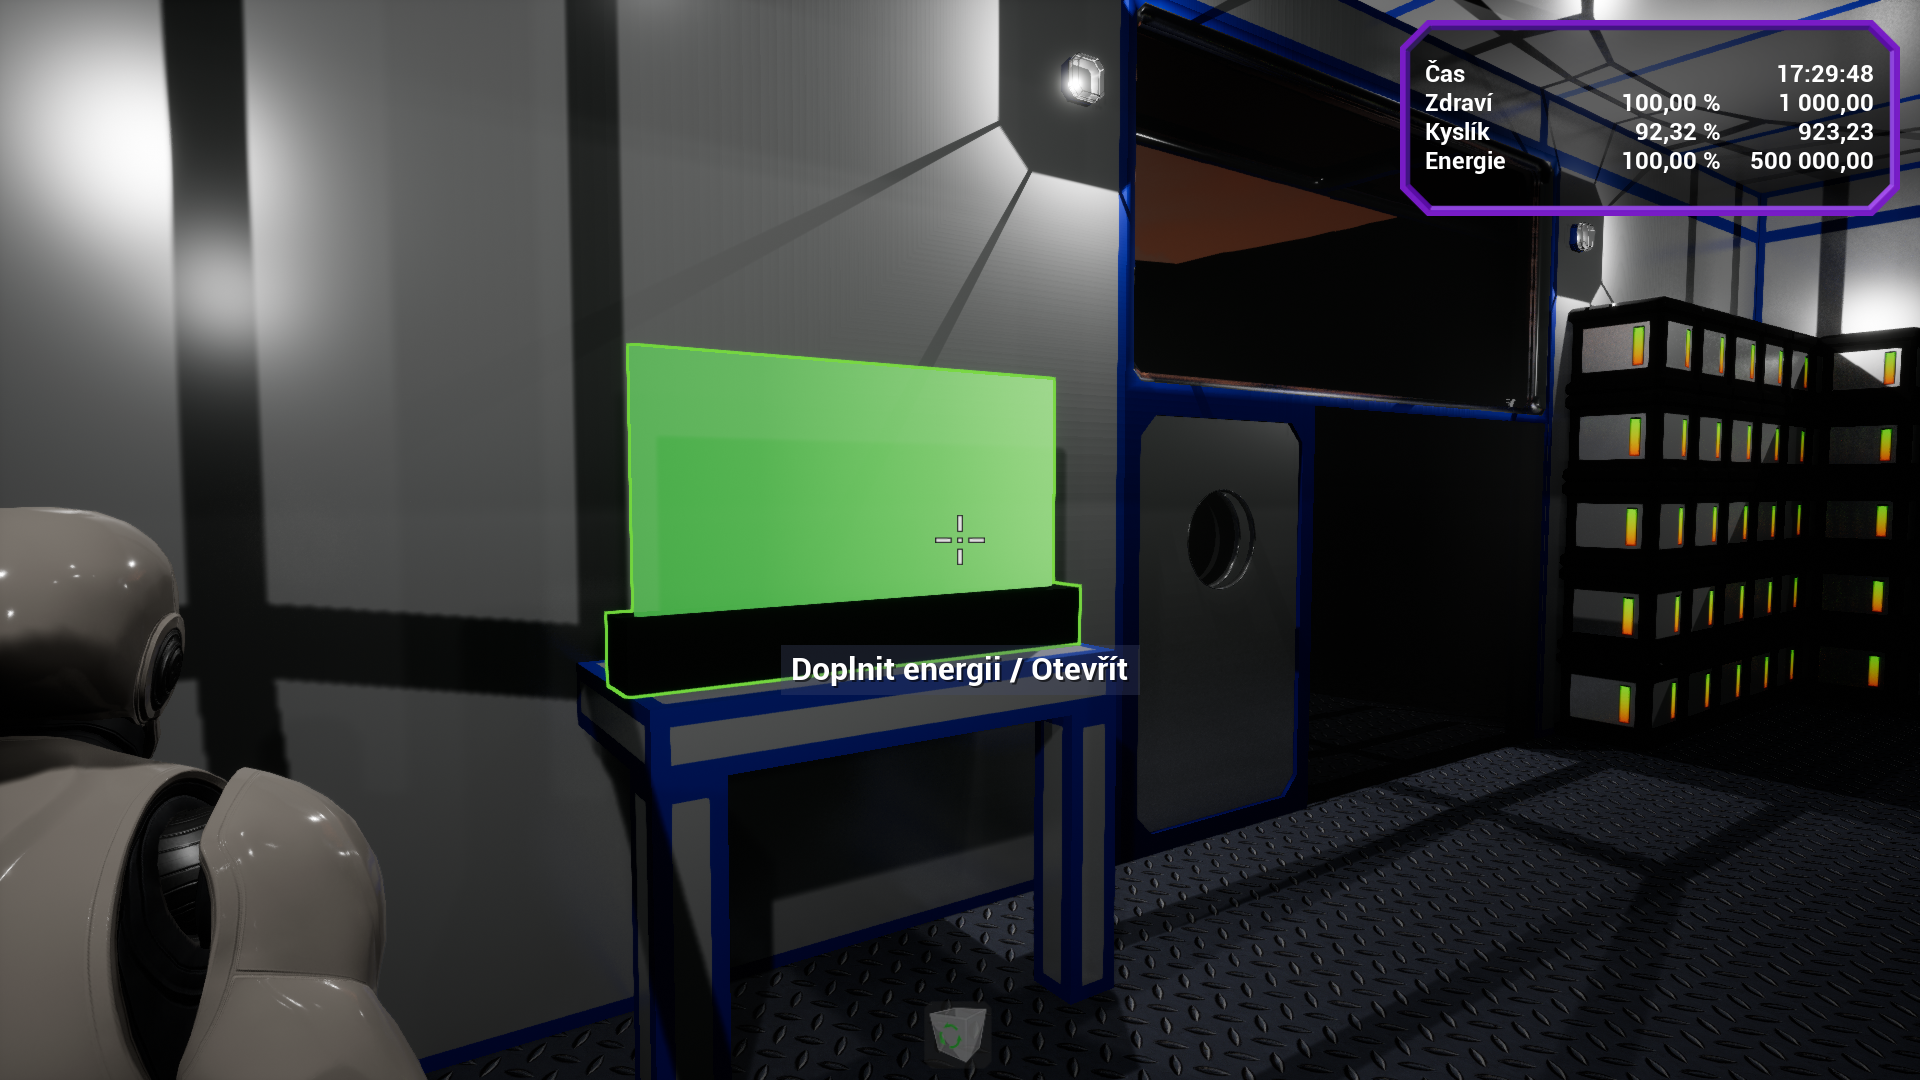
\includegraphics[ width=140mm]{../img/user/terminal/0terminalOverall}

\caption{Terminál - ve hře}
\label{fig:user_terminal_0terminalOverall}

\end{figure}

\FloatBarrier

V \textit{horní} části je vidět selektor obrazovky. Jeho rozkliknutím (více v obrázku \ref{fig:user_terminal_3terminalCtorSelector}) je možné zvolit výchozí obrazovku, nebo jeden z \textbf{Konstruktoru objektů}, které jsou v dispozici v síti.




\begin{figure}[!ht]\centering
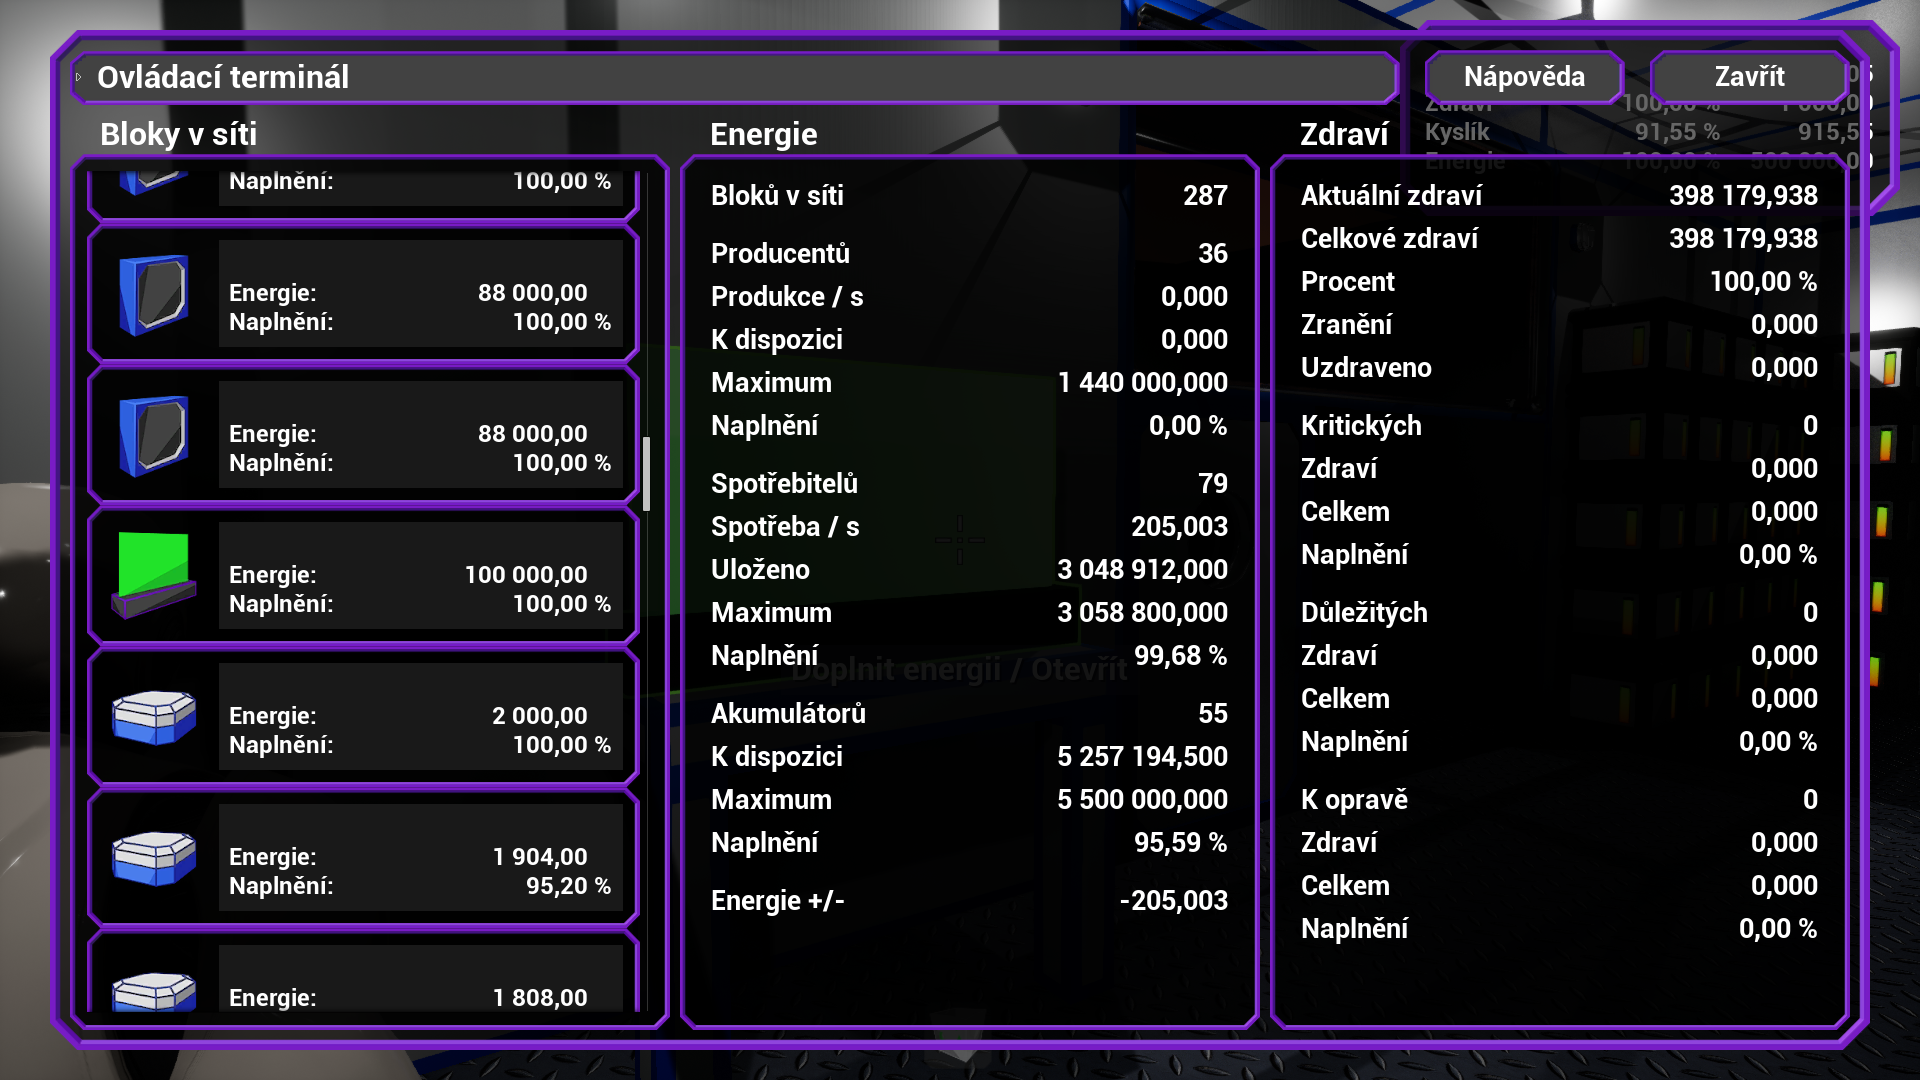
\includegraphics[ width=140mm]{../img/user/terminal/1terminalInfo}

\caption{Terminál - výchozí obrazovka}
\label{fig:user_terminal_1terminalInfo}

\end{figure}

\FloatBarrier
V \textit{levé} části je vidět seznam význačných bloků. \textit{Uprostřed} jsou vidět energetické informace o síti. \textit{Vpravo} je pak možné sledovat aktuální zdravotní stav sítě a bloků v síti.

Tlačítkem \textbf{Nápověda} je možné zobrazit informace o ovládání hry a přiřazených klávesách pro jednotlivé úkony.

\begin{figure}[!ht]\centering
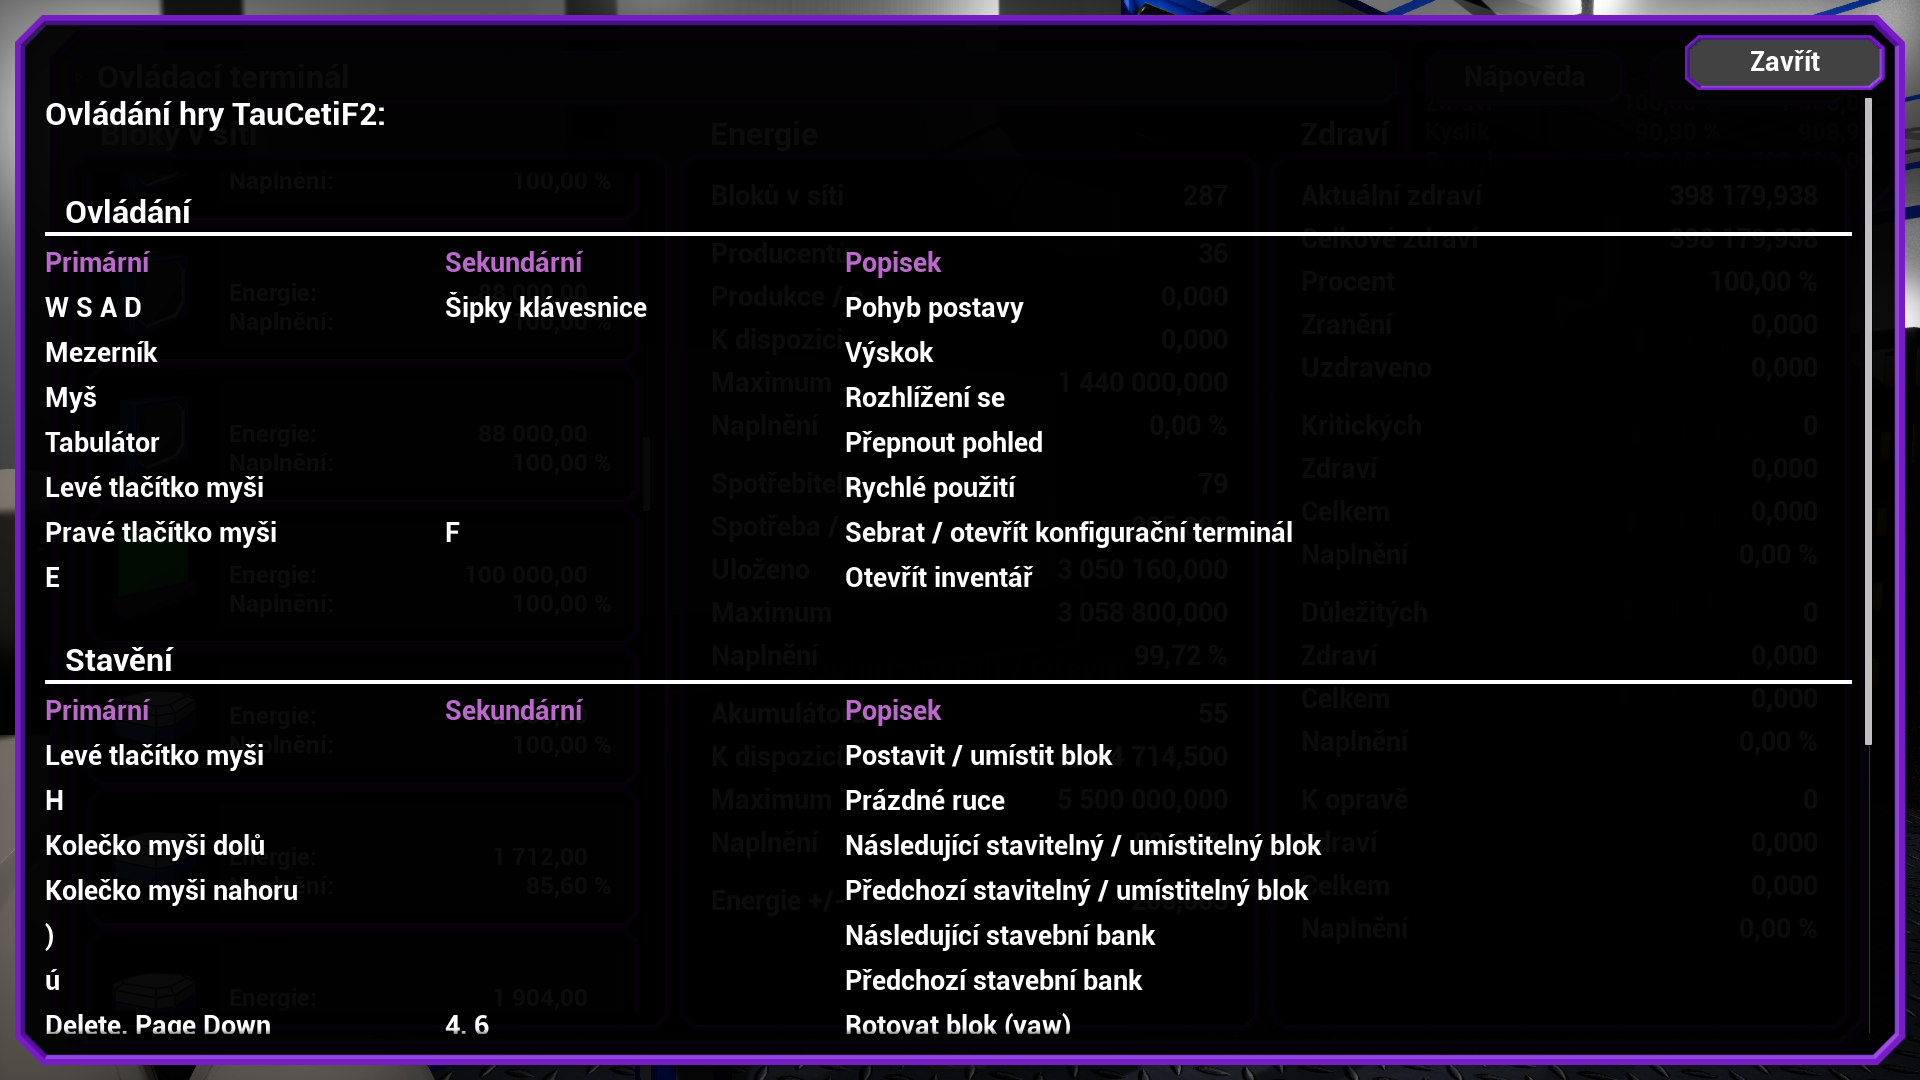
\includegraphics[ width=140mm]{../img/user/terminal/2terminalHelp}

\caption{Terminál - nápověda}
\label{fig:user_terminal_2terminalHelp}

\end{figure}

\FloatBarrier

Selektor dostupných obrazovek:

\begin{figure}[!ht]\centering
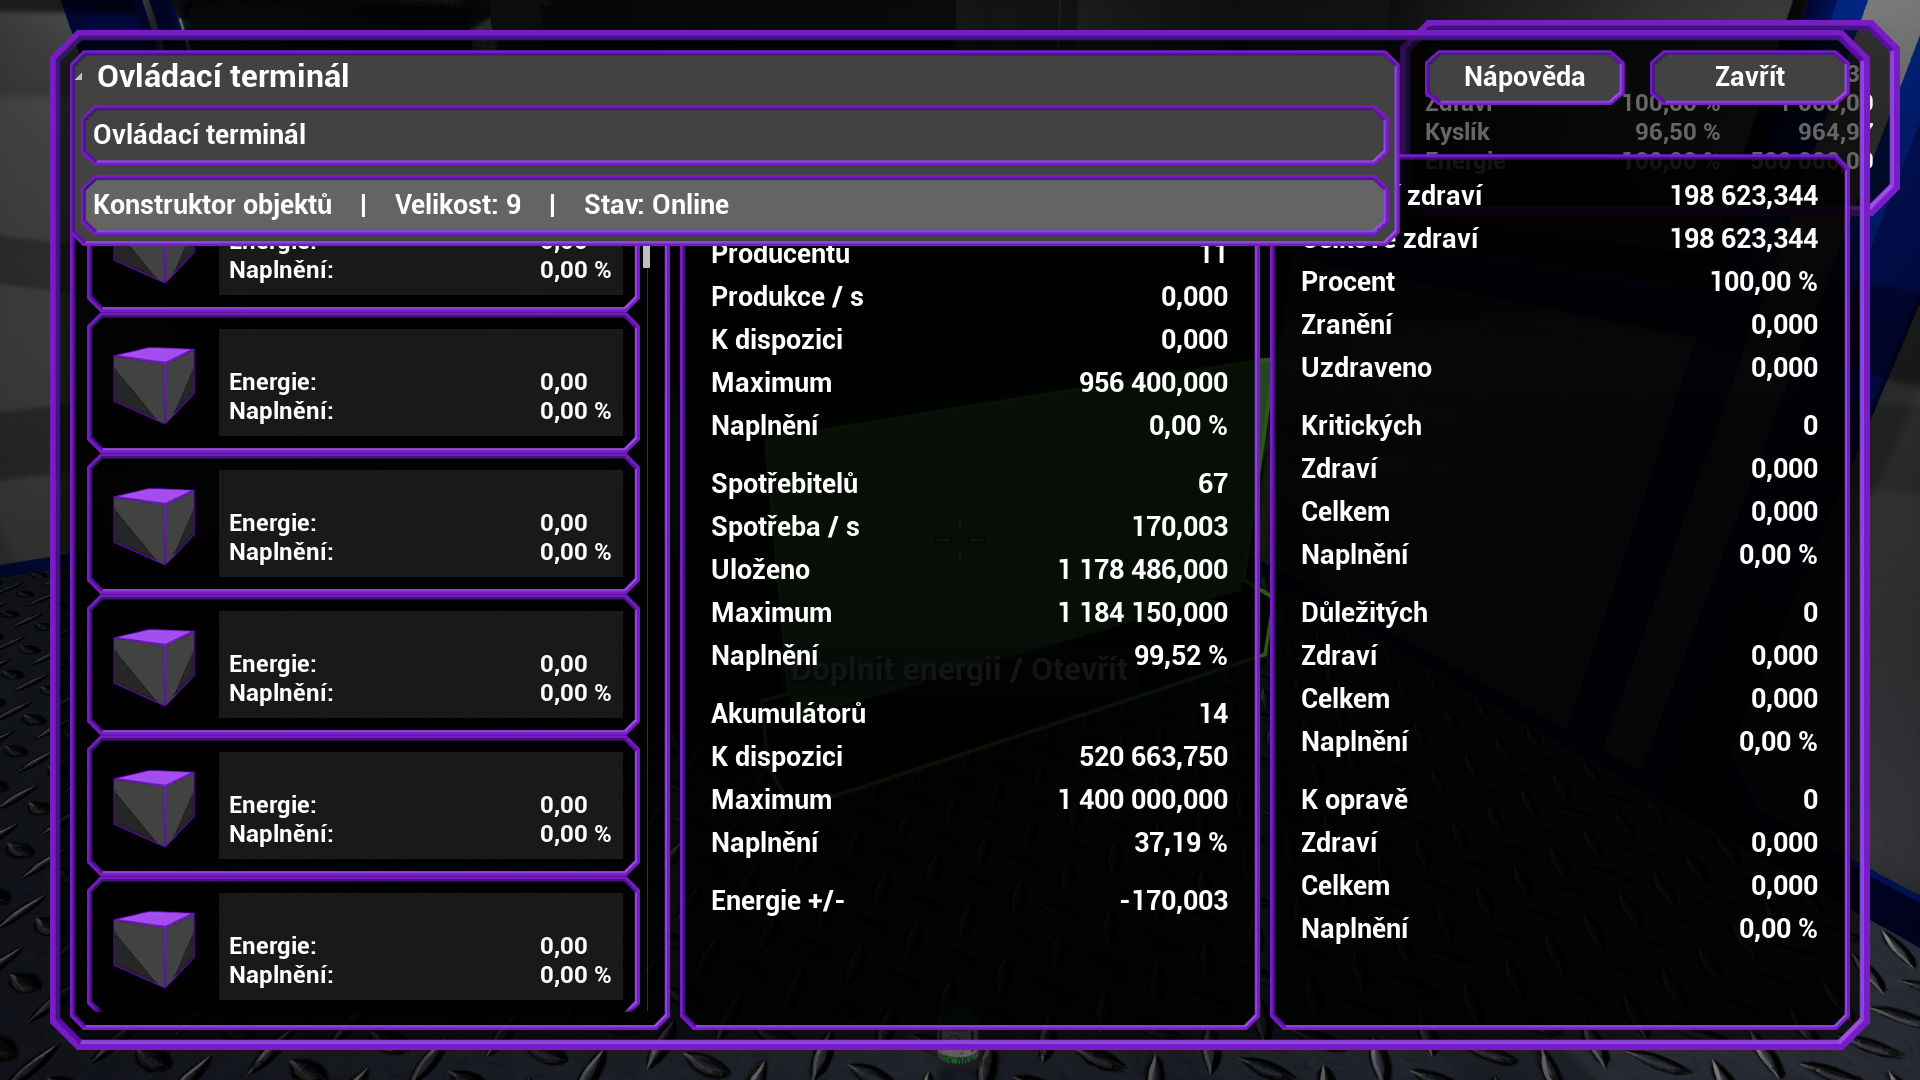
\includegraphics[ width=140mm]{../img/user/terminal/3terminalCtorSelector}

\caption{Terminál - selektor obrazovek}
\label{fig:user_terminal_3terminalCtorSelector}

\end{figure}

\FloatBarrier

Pokud vybereme \textbf{Konstruktor objektů}, vidíme seznam dostupných bloků, které můžeme zkonstruovat. Pokud to pro některé nelze (třeba z důvodu omezení velikosti - konstruktor je na daný objekt příliš malý), blok není aktivní a nelze ho zvolit.


\begin{figure}[!ht]\centering
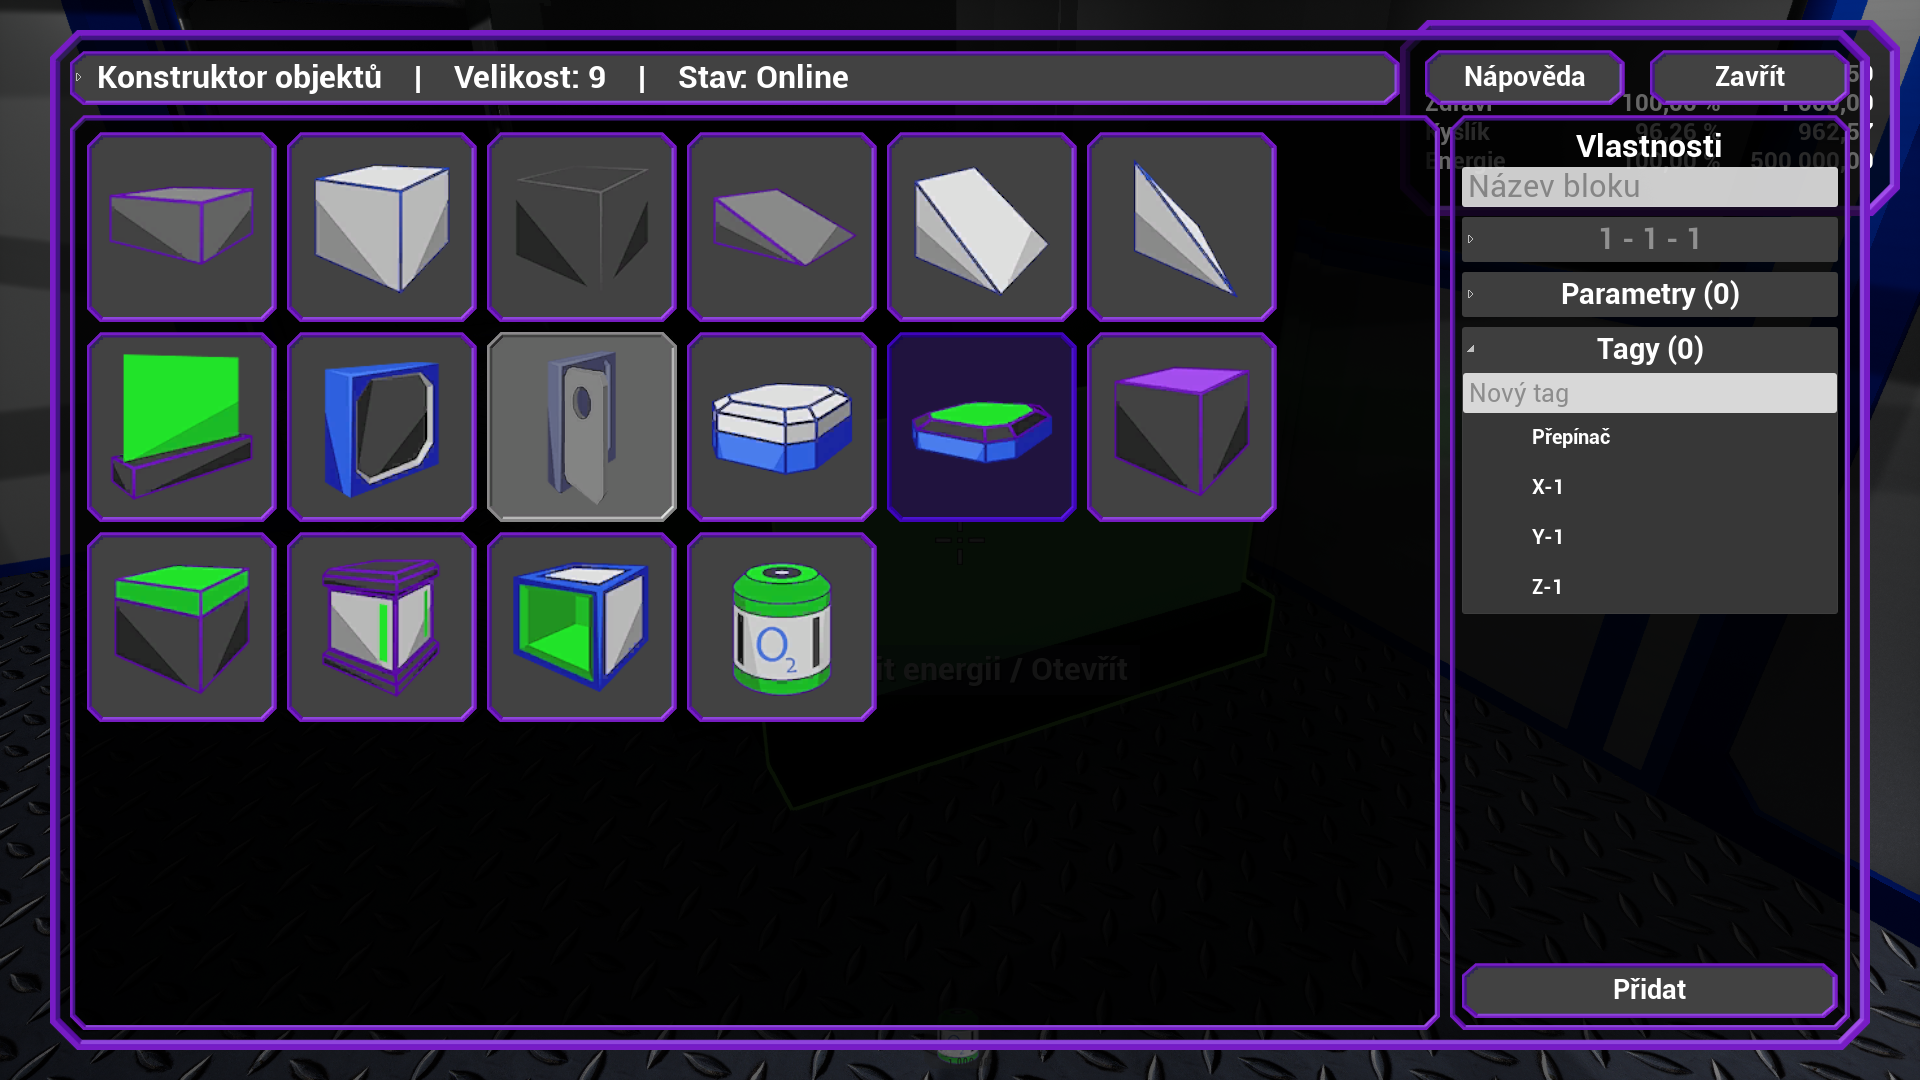
\includegraphics[ width=140mm]{../img/user/terminal/4builderSmall}

\caption{Terminál - konstruktor objektů}
\label{fig:user_terminal_4builderSmall}

\end{figure}

\FloatBarrier

V sekci \textit{Nastavení} je možné kromě tagů definovat i požadovanou velikost a to až do velikosti konstruktoru, nebo globálního omezení 20 násobku základní kostky.

\begin{figure}[!ht]\centering
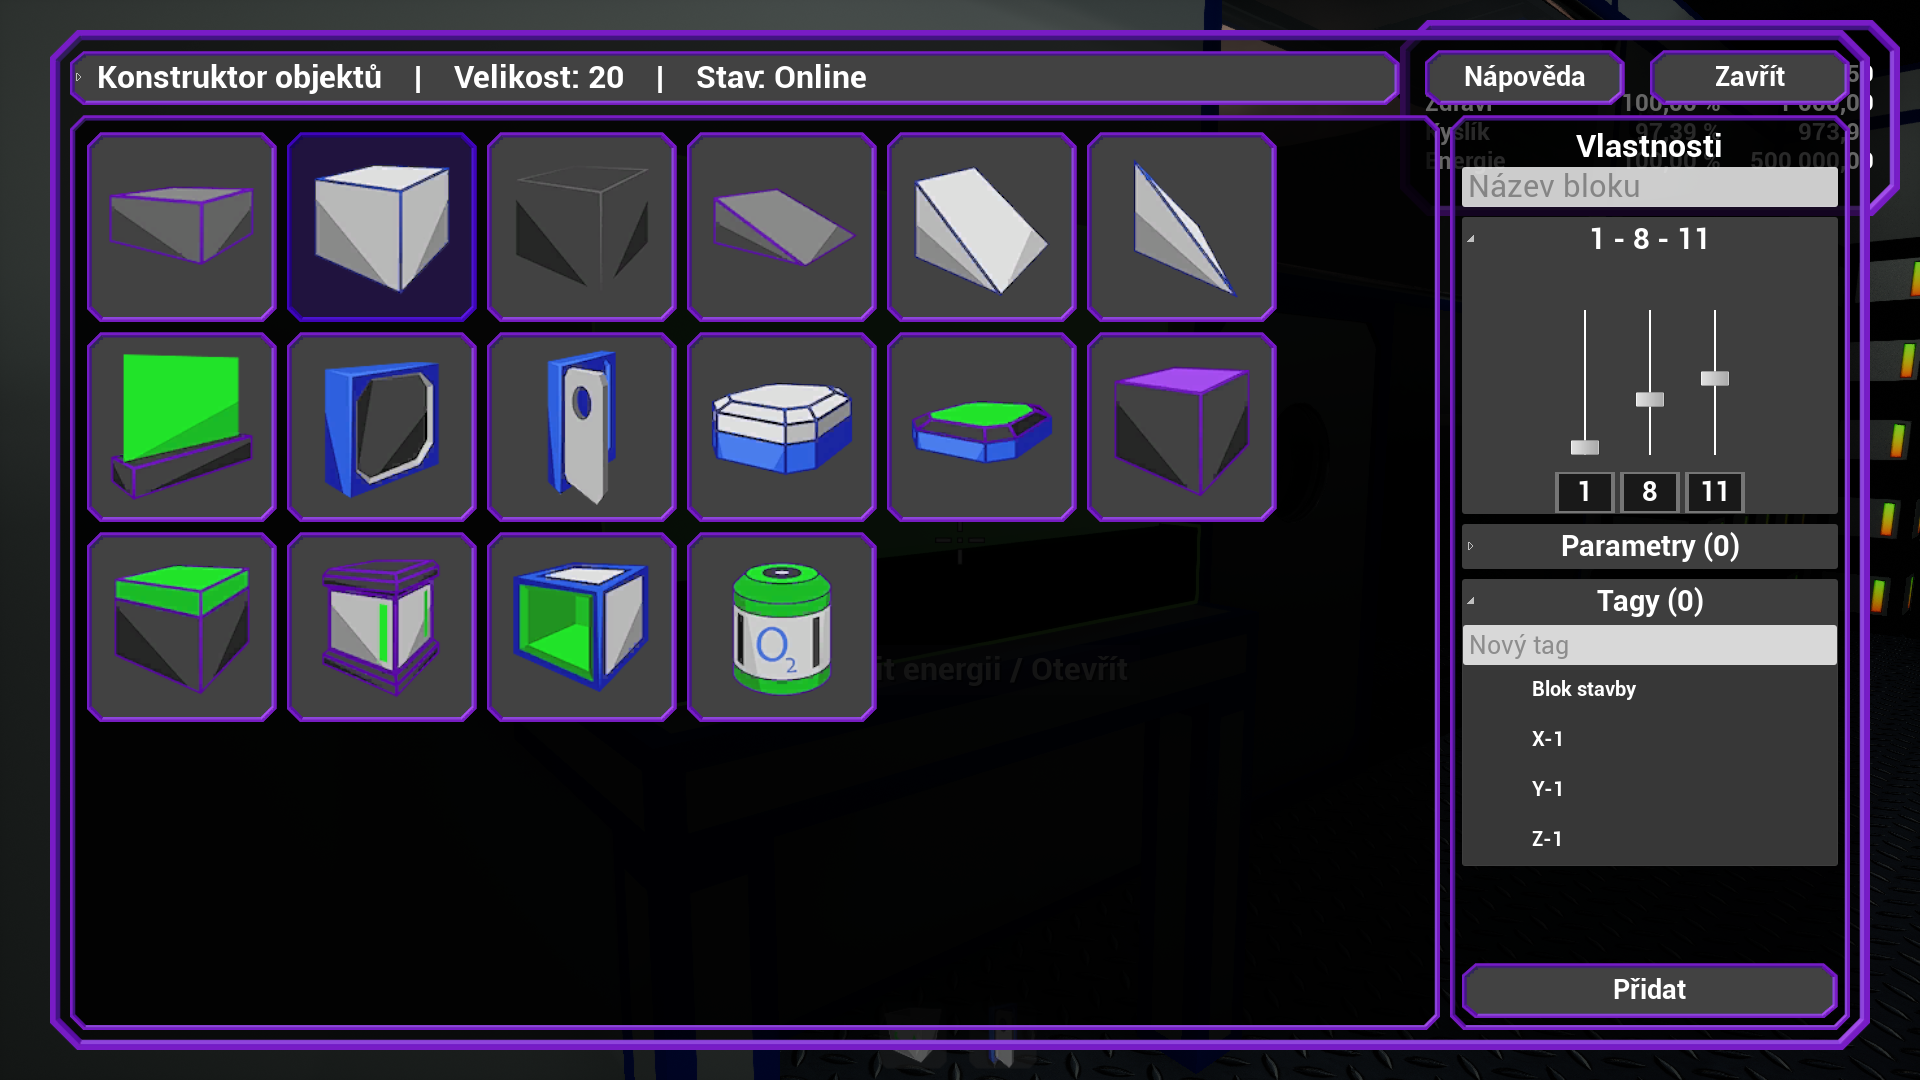
\includegraphics[ width=140mm]{../img/user/terminal/5builderSize}

\caption{Terminál - Nastavení velikosti}
\label{fig:user_terminal_5builderSize}

\end{figure}

\FloatBarrier

Některé bloky, třeba \textbf{Dveře} požadují dodatečné parametry, které ovlivňují jejich výsledné chování. V našem případě to je smysl otevírání dveří při čelním pohledu. Na obrázku je vidět stav po rozkliknutí.

\begin{figure}[!ht]\centering
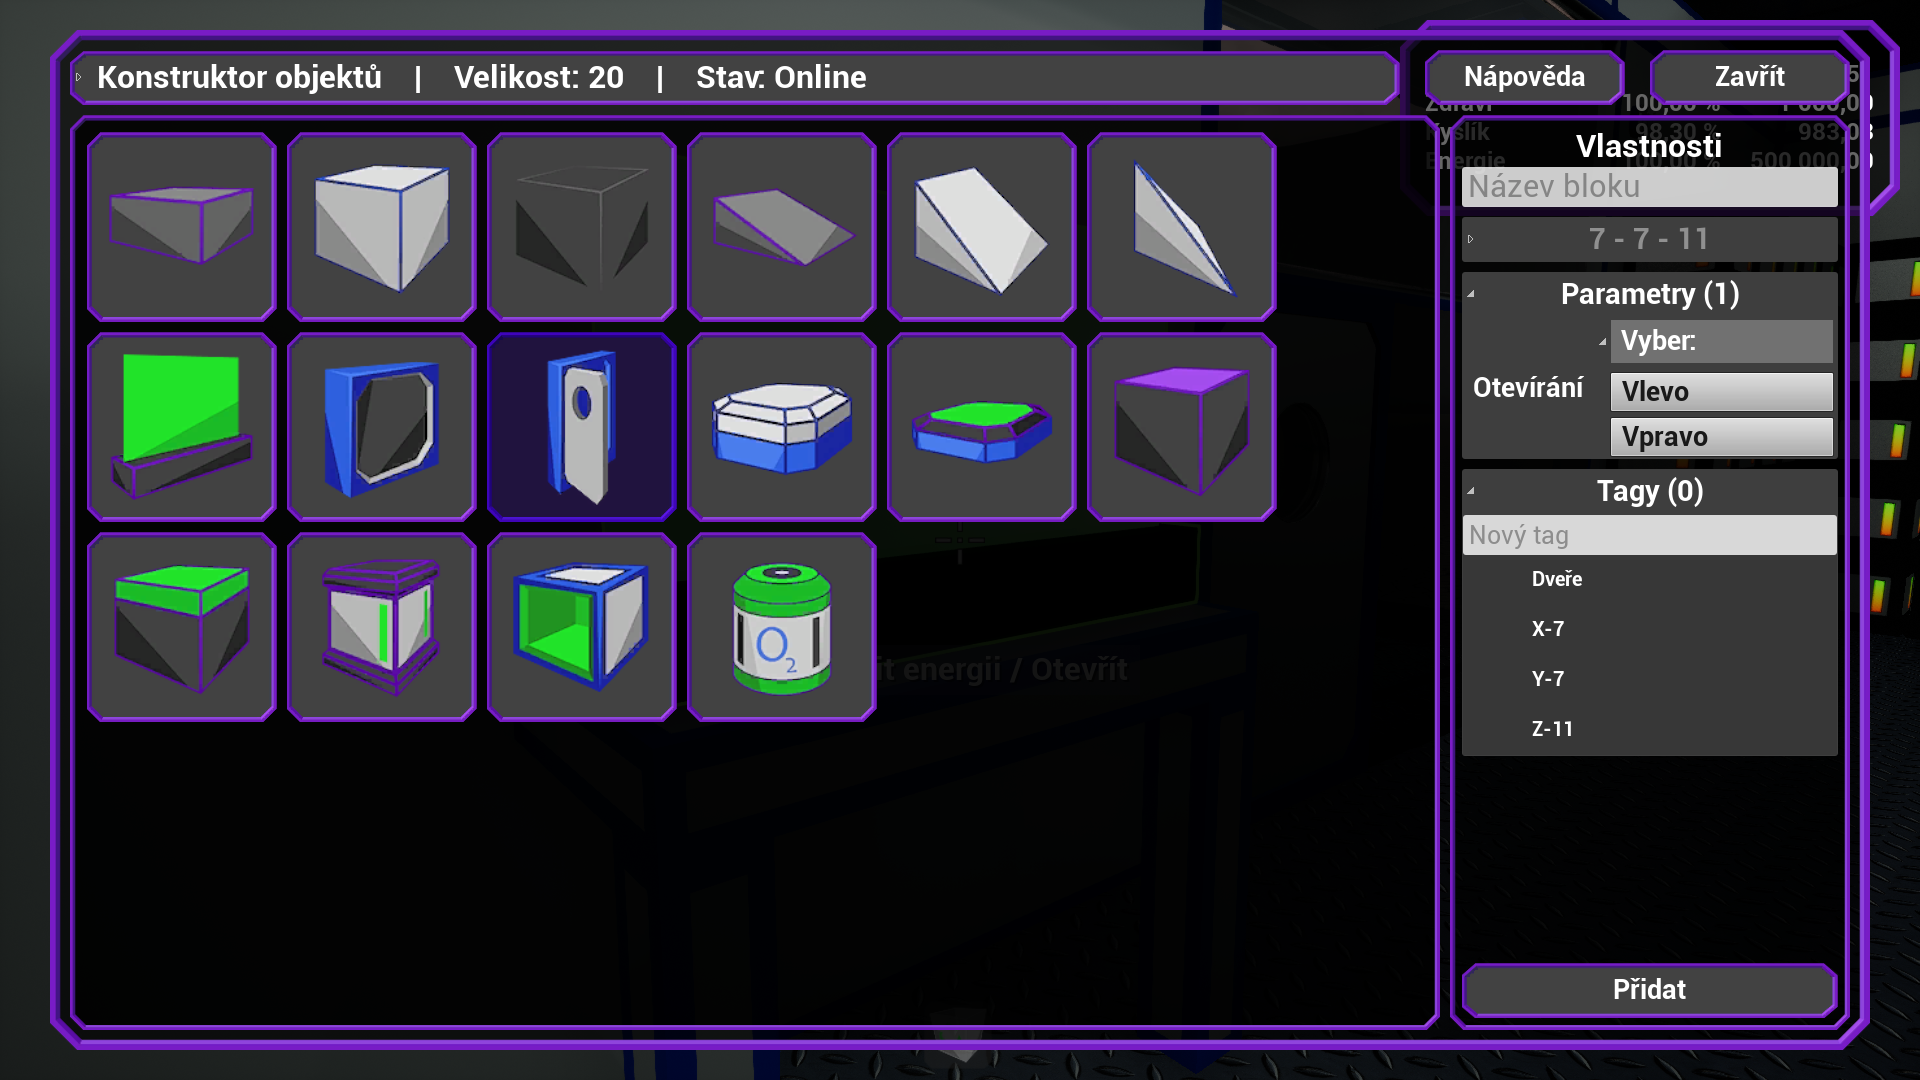
\includegraphics[ width=140mm]{../img/user/terminal/6builderParams}

\caption{Terminál - Nastavení parametrů}
\label{fig:user_terminal_6builderParams}

\end{figure}

\FloatBarrier